%\documentclass[a4paper,10.5pt]{report}
\documentclass[a4paper,10.5pt]{article}

\usepackage{booktabs}
\usepackage{epsfig}
\usepackage{amsmath}
\usepackage{rotating}

% Title Page
\textwidth 15 true cm
\textheight 25 true cm
%\headheight  14pt
%\headsep    16pt
%\footskip   27pt
%\marginparsep 10pt
%\marginparwidth  100pt
\def\marginset#1#2{
\setlength{\oddsidemargin}{#1}
\iffalse
\reversemarginpar
\addtolength{\oddsidemargin}{\marginparsep}
\addtolength{\oddsidemargin}{\marginparwidth}
\fi

  \setlength{\evensidemargin}{0mm}
\iffalse
\addtolength{\evensidemargin}{\marginparsep}
\addtolength{\evensidemargin}{\marginparwidth}
\fi

  % \paperwidth = h + \oddsidemargin+\textwidth+\evensidemargin + h
\setlength{\hoffset}{\paperwidth}
\addtolength{\hoffset}{-\oddsidemargin}
\addtolength{\hoffset}{-\textwidth}
\addtolength{\hoffset}{-\evensidemargin}
\setlength{\hoffset}{0.5\hoffset}
\addtolength{\hoffset}{-1in}           % h = \hoffset + 1in

  \setlength{\voffset}{-1in}             % 0 = \voffset + 1in
\setlength{\topmargin}{\paperheight}
\addtolength{\topmargin}{-\headheight}
\addtolength{\topmargin}{-\headsep}
\addtolength{\topmargin}{-\textheight}
\addtolength{\topmargin}{-\footskip}
\addtolength{\topmargin}{#2}
\setlength{\topmargin}{0.5\topmargin}
}

\marginset{10mm}{12mm}
      
% Title Page
\title{DVCS Simulation with SoLID-SIDIS configuration}
\author{Zhihong Ye \\ Duke University}


\begin{document}
\maketitle
\begin{abstract}
   This report quickly summaries my study of the DVCS simulation with the SoLID-SIDIS configuration. Results are preliminary and will be constantly updated.
\end{abstract}

\section{Monte Carlo Simulation Data}
  The simulated events were generated with Carlos's generator. In general, it is straightforward to generate an event with random combination of kinematic variables, $Q^{2}$, $x$, $t$ and $\phi$, and calculate the energy, momentum and angles of both the electron and photon. I implemented a slightly wider SoLID-SIDIS acceptance to judge whether both particles can be accepted by SoLID or not. In the generator, the ranges of kinematic variables I used to randomly generate events are given as:
 \begin{equation}
    \begin{align*}
    Q^{2}_{min} &= 1.0~GeV^{2},  Q^{2}_{max} = 13.0~GeV^{2}, x_{min} = 0.1, x_{max} = 0.8,\\
    t_{min} &= -2.0~GeV^{2}, t_{max} = 0.0~GeV^{2}, and \phi_{min}=0^{\circ}, \phi_{max} = 360^{\circ}.    
  \end{align*}
 \end{equation}

 We can define a phase-space factor which will be used later when evaluating the rate:
 \begin{equation}
    PSF \equiv \Delta Q^{2}\Delta x \Delta t \Delta \phi = (Q^{2}_{max}-Q^{2}_{min})\times(x_{max}-x_{min})\times(t_{max}-t_{min})\times(\phi_{max}-\phi_{min}).
    \label{psf}
 \end{equation}

 Events were simulated two energy settings, $E_{beam}$=8.8~GeV or 11~GeV, and in each setting, the total number of generated events is:
 \begin{equation}
     N_{gen} \equiv 20,000,000.
     \label{ngen}
 \end{equation}
 Only events that are in the SoLID acceptance can be stored in a ROOT file.

 In SoLID-SIDIS configuration, we detect electrons and photons at both the large-angle electromagnetic-calorimeter (LAEC) and the forward-angle electromagnetic-calorimeter (FAEC). The coverage of the detectors coded in the generator is:
  \begin{equation}
     \begin{align*}
       &6^{\circ}<=\theta_{e}<26^{\circ}, 0^{\circ}<=\phi_{e}<360^{\circ}, 0.5~GeV<=P_{e}<11~GeV,\\
       &6^{\circ}<=\theta_{\gamma}<26^{\circ}, 0^{\circ}<=\phi_{\gamma}<360^{\circ}, 0~GeV<=P_{\gamma}<11~GeV.
     \end{align*}
  \end{equation}

 The more accurate and complicated SoLID-SIDIS acceptance was applied afterward. We extracted the acceptance profiles of electrons and neutral particles (e.g. photons) from our SoLID GEANT4 simulation which contains the magnetic filed, the realistic geometries and materials of the magnet and all detectors. The acceptance profiles are basically the 2-D histograms of momentum .vs. polar angle (i.e., $P_{e}.vs.\theta_{e}$) without weighted by cross sections. Simply speaking, the acceptance value is equal to one if the particle is within the acceptance. For electrons, the acceptance has a distribution from 0 to 1 at the edge of the phase space and also depends on the momentum and angles. Because we will detect both electron and photon and form the coincidence, the overall acceptance for one event is given as:
 \begin{equation}
     A = (ele\_accpt\_fa + ele\_accpt\_la) \times (pho\_accpt\_fa + pho\_accpt\_la),
    \label{accpt}
 \end{equation}
where $ele(pho)\_accpt\_fa(la)$ is the acceptance value of an electron (photon) at FAEC (LAEC). 
% 
% Fig.~\ref{ele_acc} and Fig.~\ref{pho_acc} give the coverage of momentum and angle for electrons and photons in FAEC and LAEC at 11~GeV. Fig.~\ref{neut_acc} shows the distributions of undetected neutrons.  Fig.~\ref{kin_cor_8} and Fig.~\ref{kin_cor_11} are the coverage of some important physics variables.
% 
%  \begin{figure}[!ht]
%  \begin{center}
%   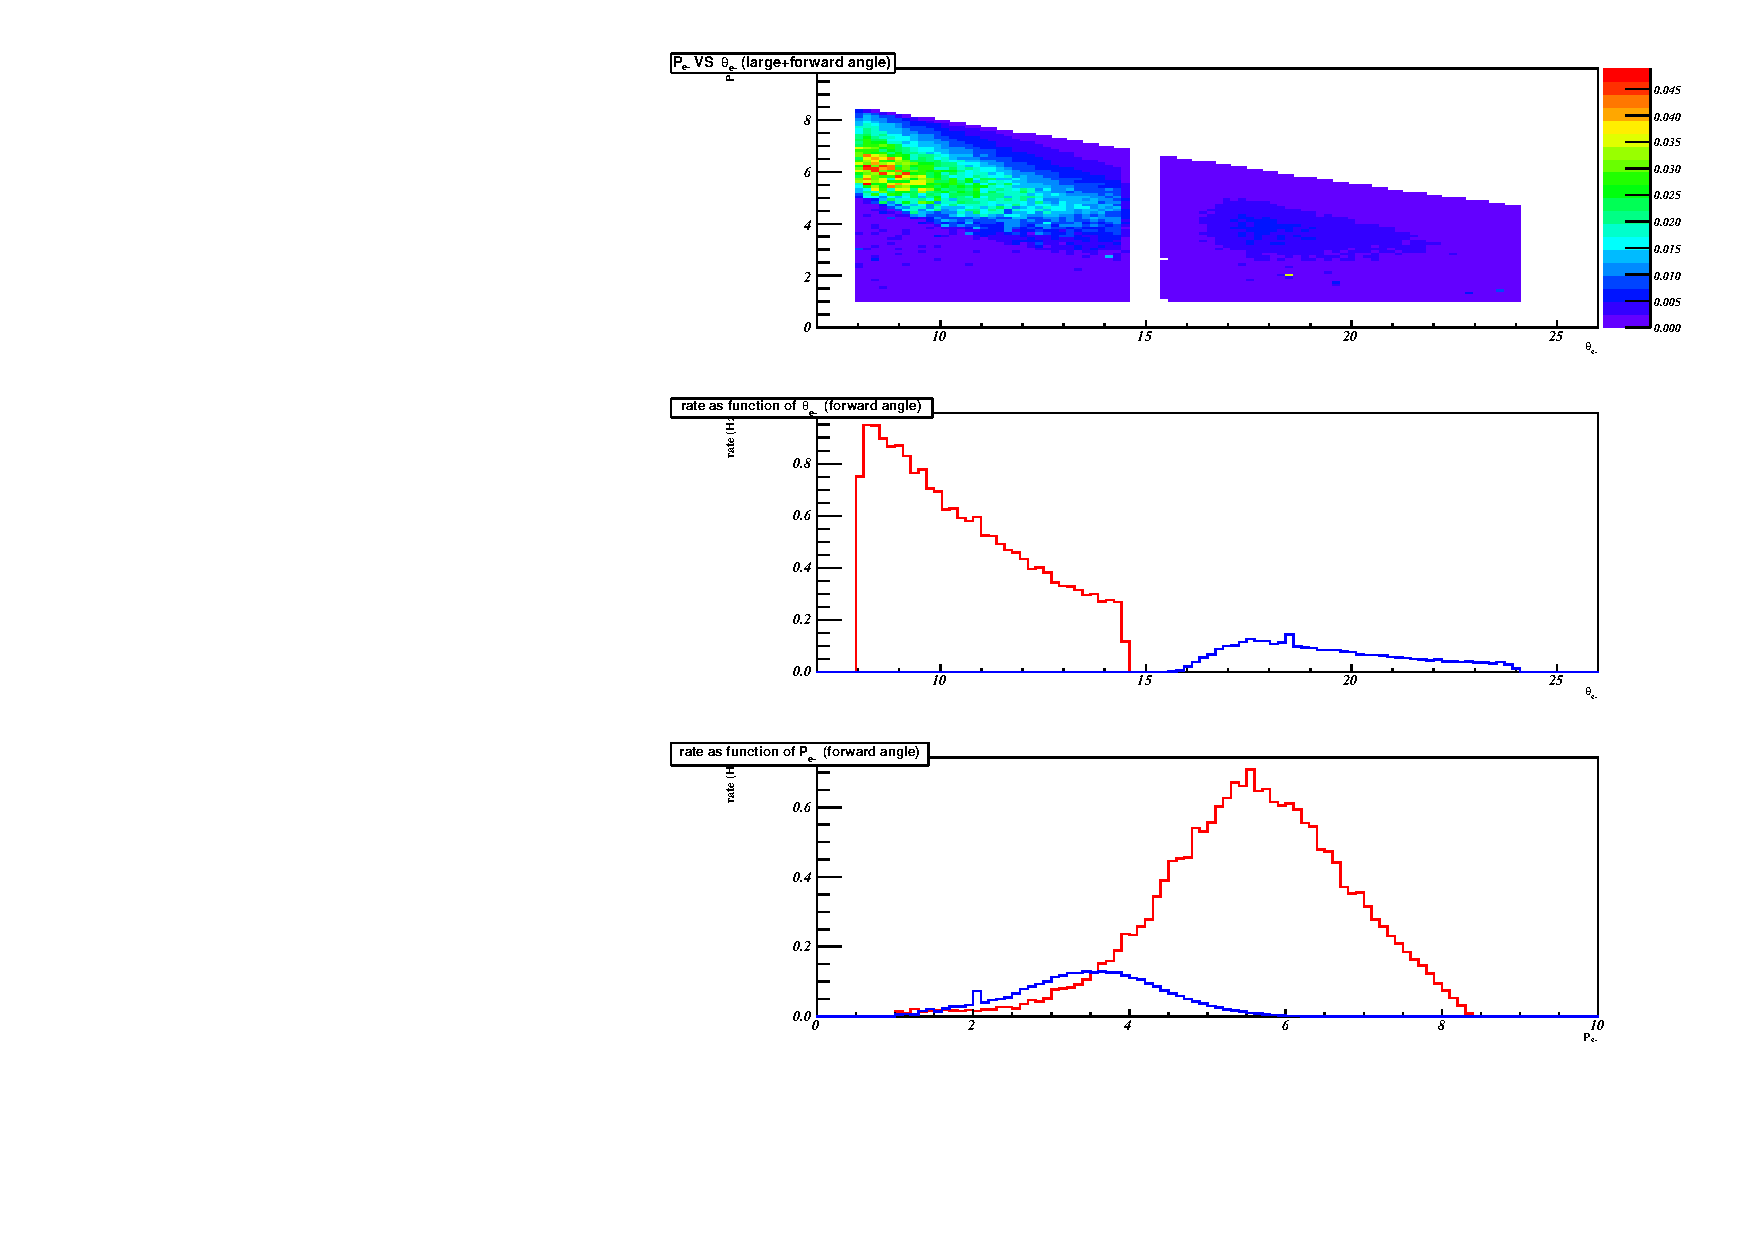
\includegraphics[width=0.6\textwidth]{./figures/CLEO_DVCS_n_11_Electron.pdf}
%   \caption[Momentum and angle coverage for electrons]{\footnotesize{Momentum and angle coverage for electrons. The top plot is the 2D histograms of $P_{e}~vs.~\theta_{e}$. The middle and bottom give the 1D $P_{e}$ and $\theta_{e}$ distributions, where the distribution at FAEC is given in blue line and the one at LAEC is given in red line. The color in the top plot and the value on the Y-axis of the bottom two plots reveal the normalized rate in Hz.}}
%   \label{ele_acc}
%  \end{center}
% \end{figure}
% 
% \begin{figure}[!ht]
%  \begin{center}
%   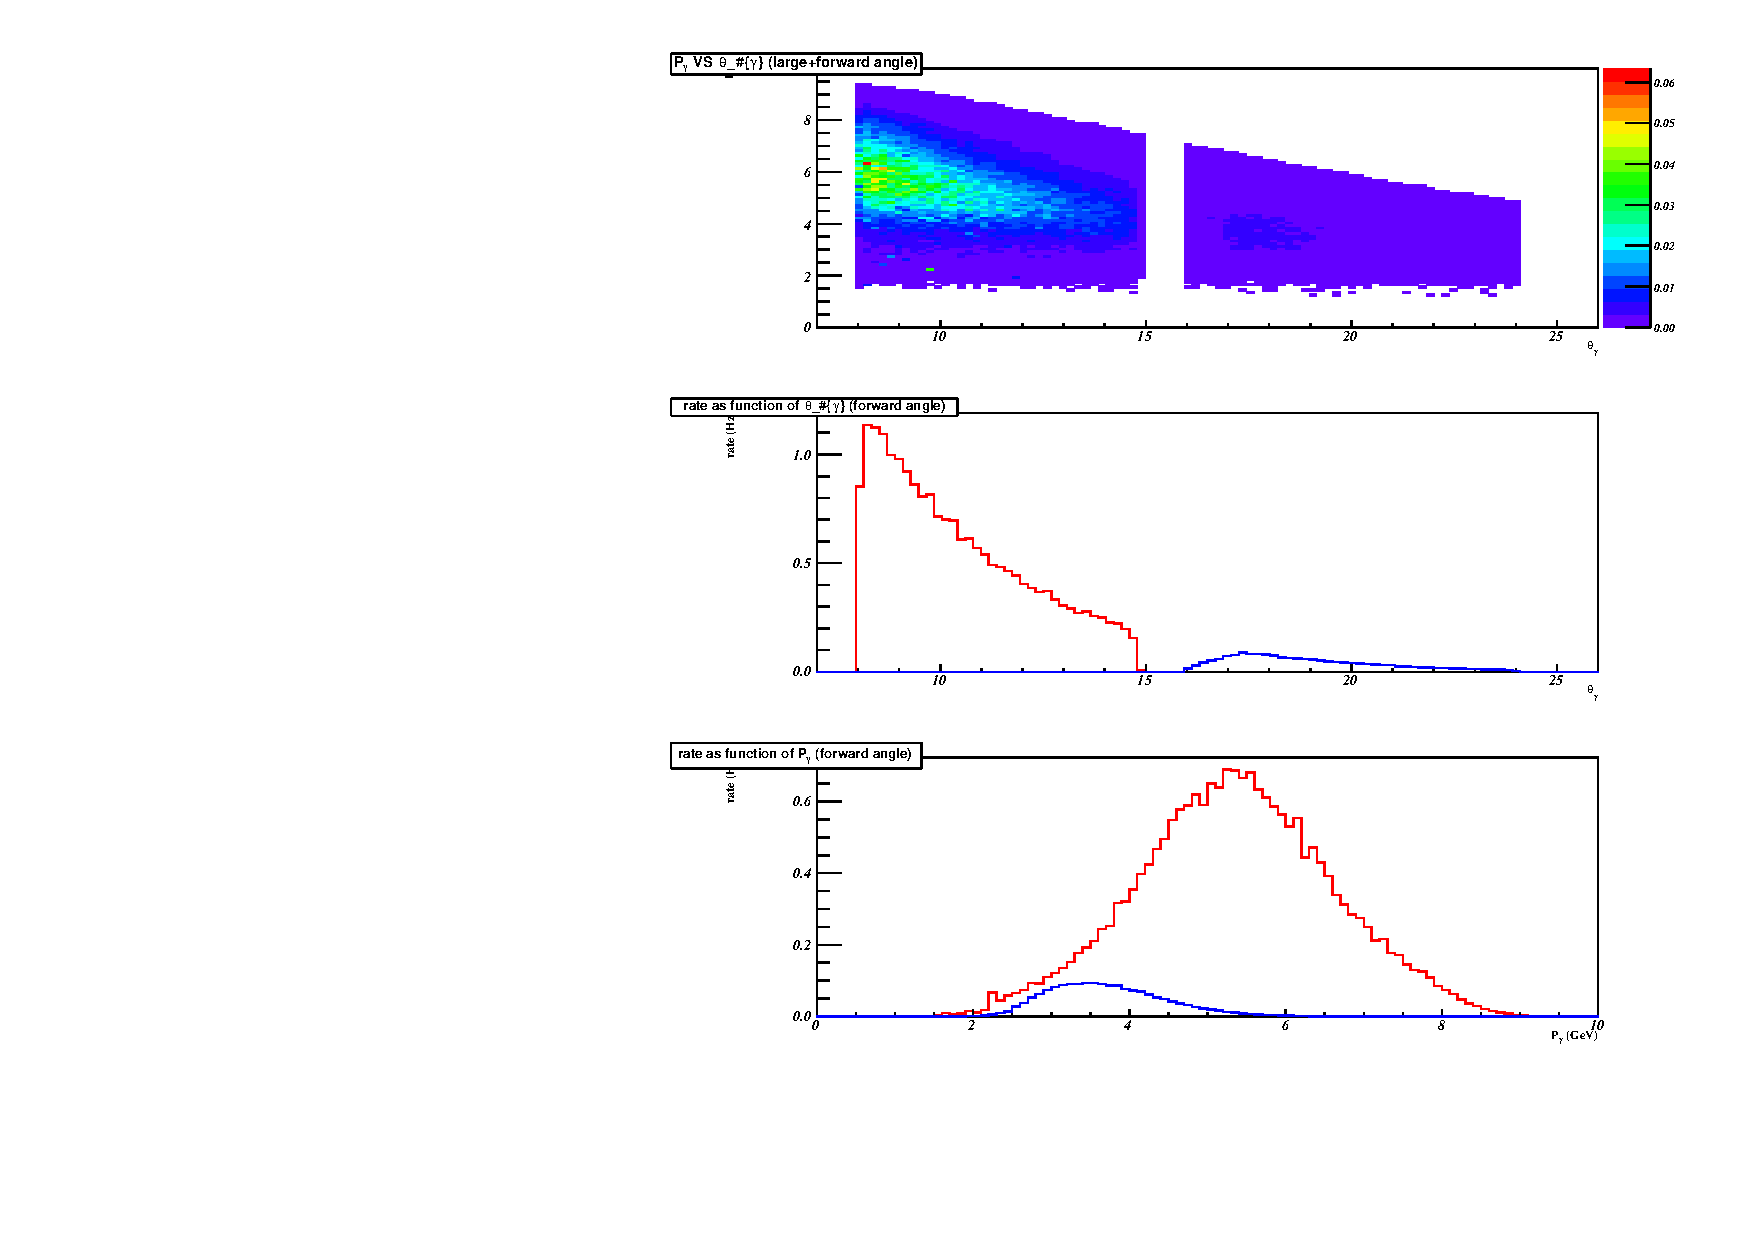
\includegraphics[width=0.6\textwidth]{./figures/CLEO_DVCS_n_11_Photon.pdf}
%   \caption[Momentum and angle coverage for photons]{\footnotesize{Momentum and angle coverage for photons. The top plot is the 2D histograms of $P_{\gamma}~vs.~\theta_{\gamma}$. The middle and bottom give the 1D $P_{\gamma}$ and $\theta_{\gamma}$ distributions, where the distribution at FAEC is given in blue line and the one at LAEC is given in red line. The color in the top plot and the value on the Y-axis of the bottom two plots reveal the normalized rate in Hz.}}
%   \label{pho_acc}
%  \end{center}
% \end{figure}
% 
% \begin{figure}[!ht]
%  \begin{center}
%   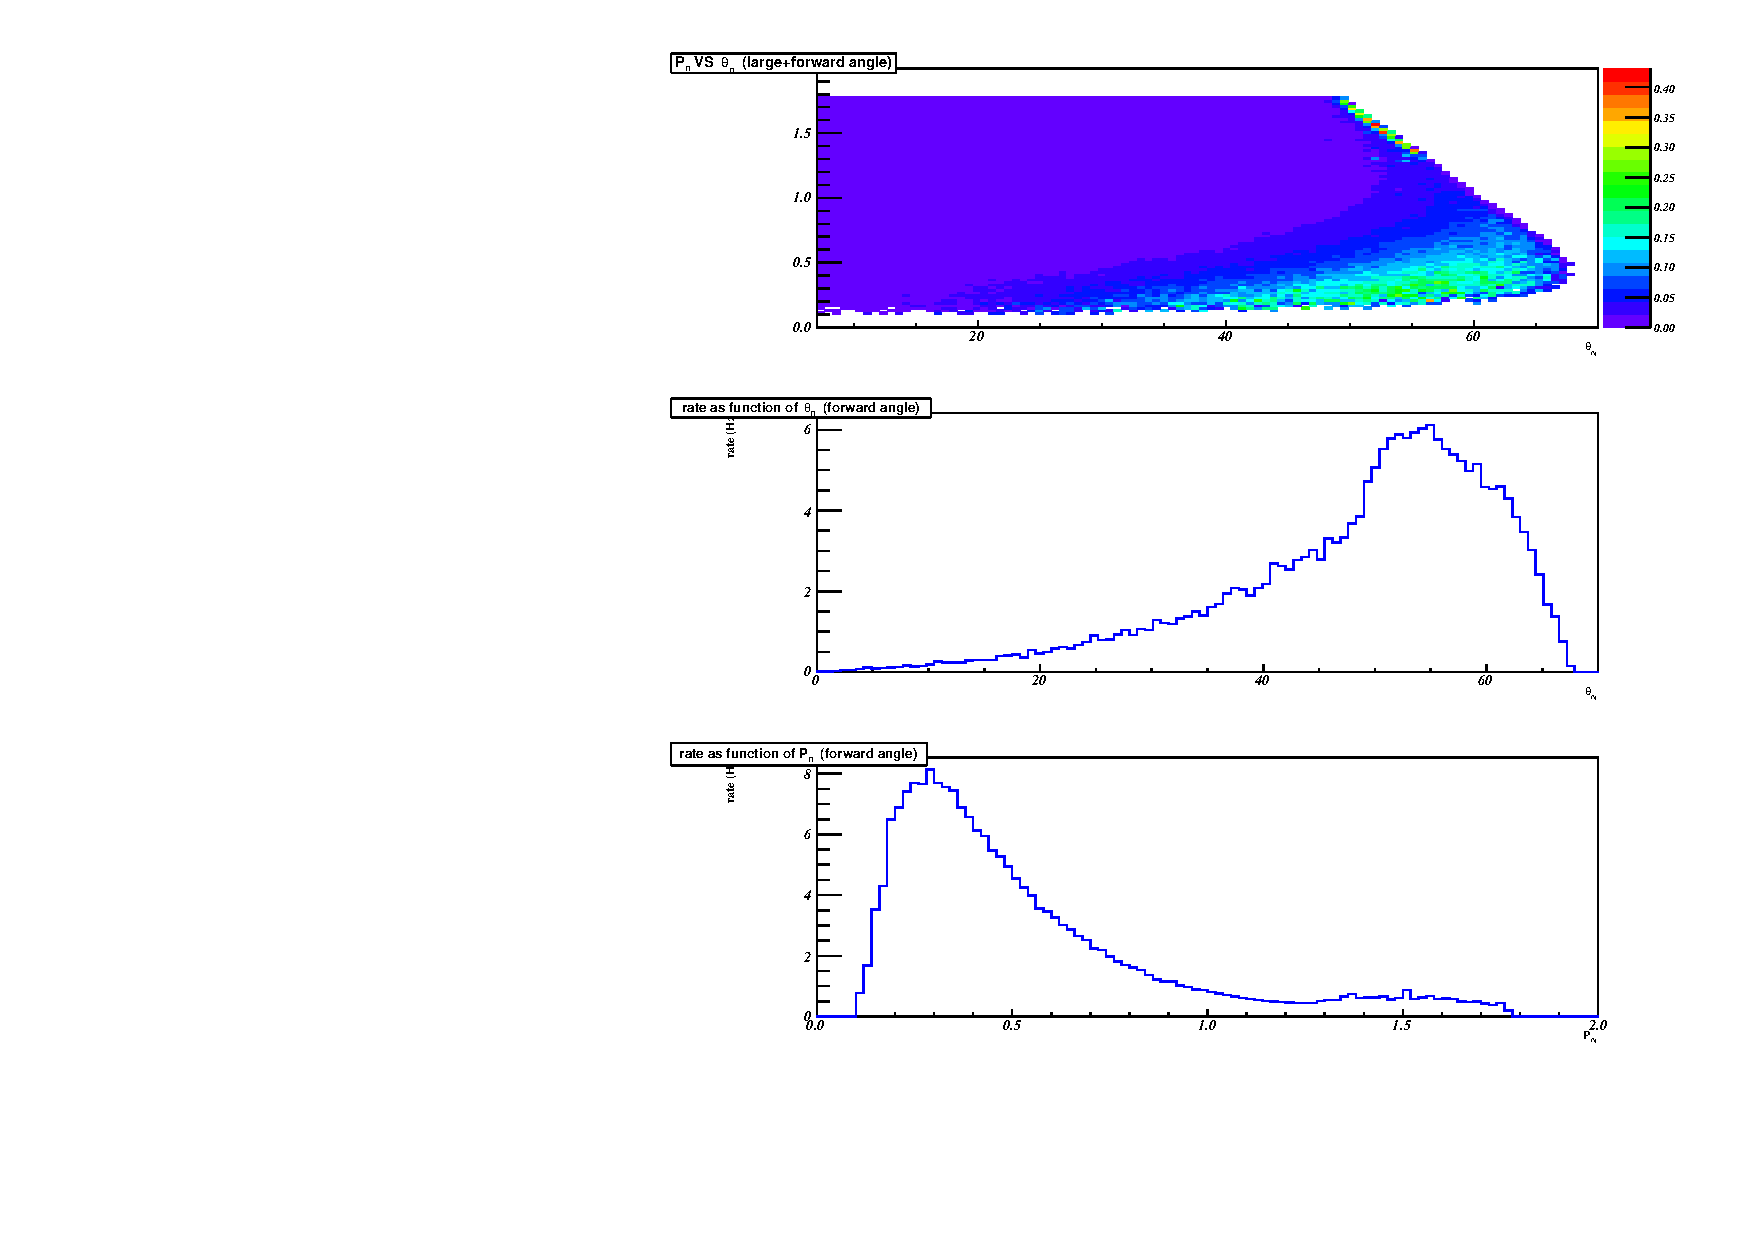
\includegraphics[width=0.6\textwidth]{./figures/CLEO_DVCS_n_11_Hadron.pdf}
%   \caption[Momentum and angle coverage for neutrons]{\footnotesize{Momentum and angle coverage for neutron which won't be detected by SoLID detectors. The top plot is the 2D histograms of $P_{n}~vs.~\theta_{n}$. The middle and bottom give the 1D $P_{n}$ and $\theta_{n}$ distributions, where the distribution at FAEC is given in blue line and the one at LAEC is given in red line.}}
%   \label{neut_acc}
%  \end{center}
% \end{figure}
% \begin{figure}[!ht]
%  \begin{center}
%   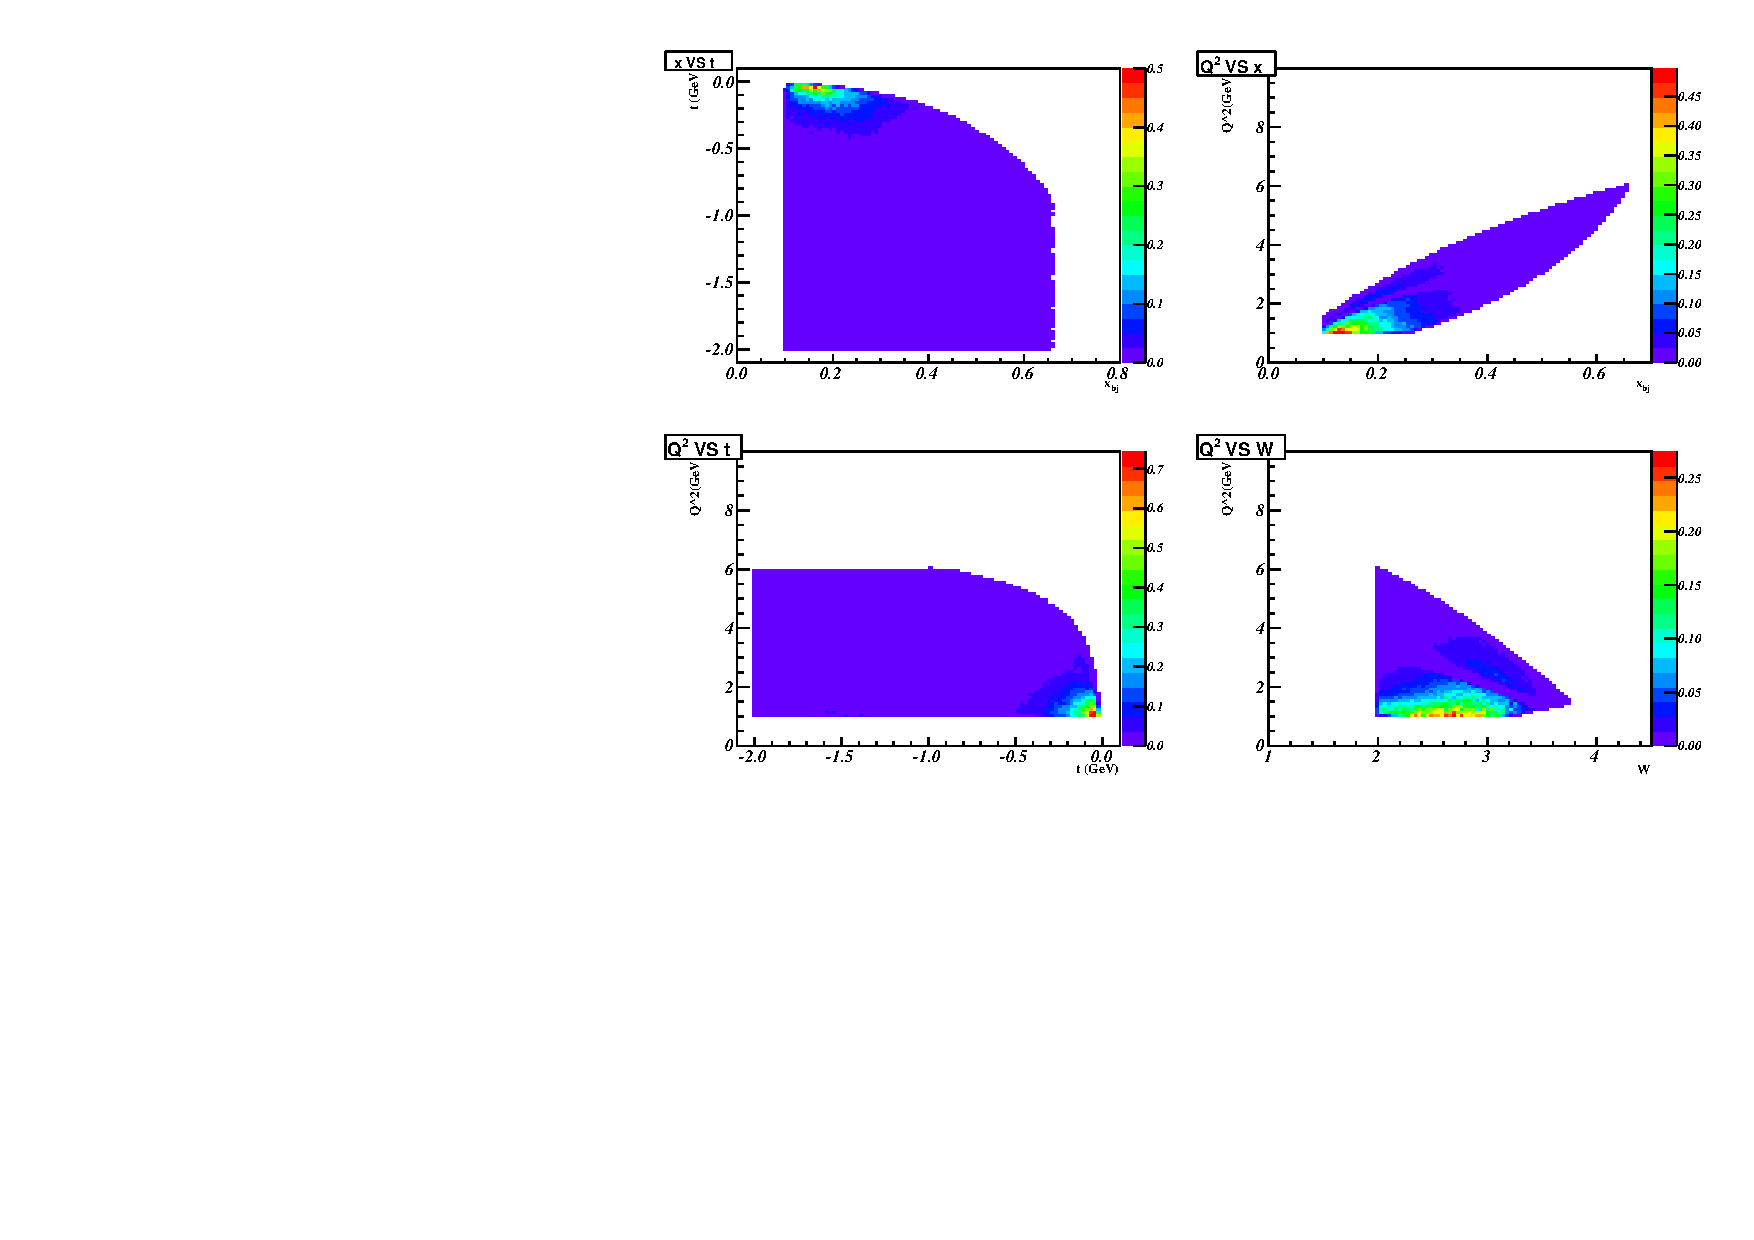
\includegraphics[width=0.6\textwidth]{./figures/CLEO_DVCS_n_8_Total2.pdf}
%   \caption[The coverage of important physics variables at $E_{beam}=8.8~GeV$]{\footnotesize{The coverage of important physics variables at $E_{beam}=8.8~GeV$}}
%   \label{kin_cor_8}
%  \end{center}
% \end{figure}
% 
% \begin{figure}[!ht]
%  \begin{center}
%   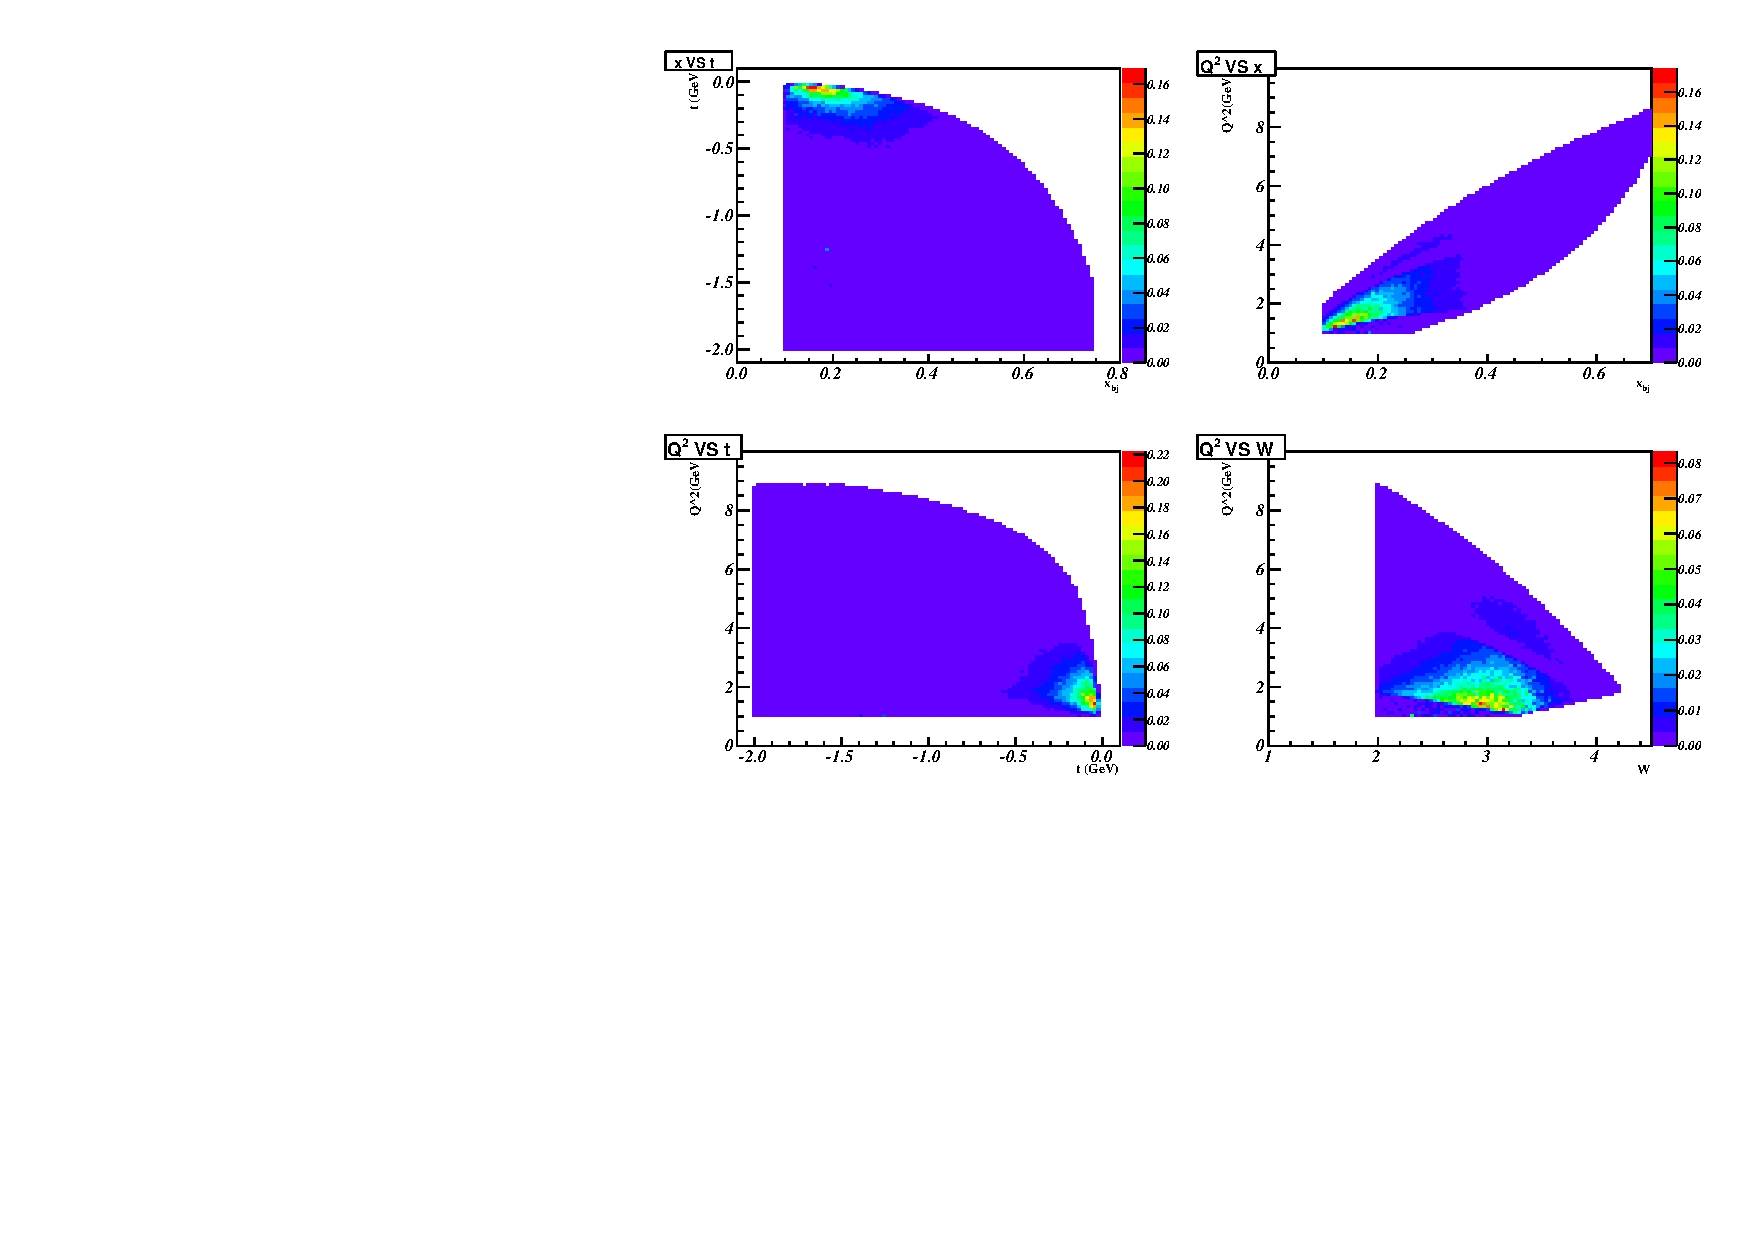
\includegraphics[width=0.6\textwidth]{./figures/CLEO_DVCS_n_11_Total2.pdf}
%   \caption[The coverage of important physics variables at $E_{beam}=11~GeV$]{\footnotesize{The coverage of important physics variables at $E_{beam}=11~GeV$}}
%   \label{kin_cor_11}
%  \end{center}
% \end{figure}
% 

\section{VGG Cross Section Model}
  (Note: More introduction about VGG will be added later.)
  The VGG model is able to provide the BH+DVCS cross section with the known inputs of $Q^{2}, x, t,$ and $\phi$. In the double polarized case, the code computes four cross section values at the same time, i.e. $\sigma^{++}, \sigma^{+-}, \sigma^{-+}$, and $\sigma^{--}$, where first and second superscript ($\pm$) gives the polarization direction of the beam and the target, respectively. The unit of the cross section is in $nb\cdot GeV^{-4}\cdot rad^{-1}$ and was later converted into $cm^{2}\cdot GeV^{-4}\cdot rad^{-1}$

\begin{table}[htbp]
  \begin{center}
 \begin{tabular}{|l|c|c|c|c|}
 \toprule
                &    Min   &   Max   &   Step\\
 \midrule
  $Q^{2}$       & 1~$GeV^{2}$ & 9~$GeV^{2}$ & 1~$GeV^{2}$ \\
  $x$           & 0.05 & 0.75 & 0.05 \\
   $t$          & -2.5~$GeV^{2}$ or $t_{max}$ & 0~$GeV^{2}$ or $t_{min}$ & 0.05~$GeV^{2}$ \\
  $\phi$        & $0^{\circ}$ & $360^{\circ}$ & $15^{\circ}$ \\
 \bottomrule
 \end{tabular}
% \centering
\caption{Ranges and steps for physics variables when calculating cross sections with VGG}
\label{vgg_table}
  \end{center}
\end{table}

  The VGG code runs very slow so it is not practical to compute the cross sections in an event-by-event base. As shown in Table~\ref{vgg_table}, after determining the range and step of each variable, I created a 4D grid where in each grid point the four cross section values were computed. The polarization of the electron beam is always longitudinal (L), while there are three target polarization directions, i.e. longitudinal, transverse on x (Tx) and transverse on y (Ty). Hence there are three double-spin combinations, LL, LTx and LTy. With two energy settings, there are 6 grids I created.
  
  With these grids, I am able to search the cross section values for each simulated event created by the generator. Given an event with known values of these four variables, I searched which two grid points each variable falls into, and used the linear relationship to calculate the ``actual`` cross section value with the known values on the two grid points. For example, if the value of $\phi$ is between $\phi_{i}$ and $\phi_{i+1}$, the correction is given as:
  \begin{equation}
     cor(\phi) = 1 + \frac{\phi-\phi_{i}}{\phi_{i+1}-\phi_{i}}\frac{\sigma_{i+1}-\sigma_{i}}{\sigma_{i}}.
  \end{equation}
  Hence, there are four corrections ($cor(Q^{2}), cor(x), cor(t), cor(\phi))$) when searching cross sections for each event. A C++ script was written to perform searching and apply corrections. A random test with several events was proceeded to compare the difference between the values computed directly by VGG and searched by the script. The results show less than 0.5\% deviation but a more careful check can be done later.
 
 \section{Integrated Rate}
  \begin{table}[htbp]
  \begin{center}
 \begin{tabular}{|l|c|c|c|c|}
 \toprule
                &   \multicolumn{2}{c|}{TGVKelly} &   \multicolumn{2}{c|}{VGG}   \\                    
 \midrule
                &    8.8~GeV   &  11~GeV   &   8.8~GeV & 11~GeV\\
 \midrule
                &  \multicolumn{4}{c|}{Single Rates (Hz)}                                     \\
 \midrule

 e- (FAEC)      &  117.64      &  63.42 & 259.26 &144.67   \\
 e- (LAEC)      &  4.25        & 3.60   & 11.09 &6.73   \\
 $\gamma$ (FAEC)&  80.37       & 55.09  & 182.56 &162.27    \\
 $\gamma$ (LAEC)&  8.48        & 5.80   & 125.30 &115.54    \\
\midrule
                &   \multicolumn{4}{c|}{Coincidence Rates (Hz)}                                     \\
 \midrule
e-(FAEC)+$\gamma$(FAEC+LAEC) & 40.12 & 19.00 & 144.48  & 82.28   \\
e-(LAEC)+$\gamma$(FAEC+LAEC) & 2.08 & 1.50   &  6.25  &  3.94   \\
 \bottomrule
\end{tabular}
% \centering
\caption{Ranges and steps for physics variables when calculating cross sections with VGG}
\label{rate_table}
  \end{center}
\end{table}
    We will perform the exclusive DVCS measurement and hence it requires the coincident trigger of electrons and photons. The integrated rates given below are not corrected by the beam and target polarization, target dilution and so on. They are not corrected by the detector efficiency as well (which is about 85\% ). It will just represent what we can detect at the trigger level.
  
  The rates are calculated with the simulated events weighted by their total cross sections and acceptances. In Carlos' generator, the TGVKelly model was used to compute the unpolarized cross sections. I used these values to evaluate the rates. After generating the cross section grids, I redid the calculation with the cross sections from VGG. In the Table~\ref{rate_table}, the VGG model gives the coincidence rates which are a factor of 3 larger than the ones from TGVKelly. The biggest difference is the single photon rates at LAEC. I am looking for the reason now.
 
\section{Beam Time, Target, etc}
  Currently I assume the DVCS experiment will be in the run group of the SoLID-SIDIS and hence share the beam time of the approved experiments. The approved beam time of two energy settings are:
  \begin{equation}
     T_{8.8GeV} = 21~days, T_{11GeV} = 48~days.
     \label{beamtime}
  \end{equation}
  
  In the SoLID-SIDIS experiments, we will use transverse polarized $^{3}He$ target (neutron) and longitudinal polarized $NH3$ target (proton). In this study, I only evaluated the transverse case. With $15~nA$ beam current, the neutron luminosity in the $^{3}He$ target is:
  \begin{equation}
     L = 1\times 10^{36} cm^{-2}s^{-1}.
     \label{lumi}
  \end{equation}
  The beam polarization and the $^{3}He$ polarization are set to be $100\%$ and $60\%$, respectively. The effective neutron in $^{3}He$ is known to be close to $86.5\%$, and the dilution is estimated to be $20\%$. The total detector efficiency is assumed to be $85\%$
  
\section{Data Binning and Projections}
 The binning was performed for each energy setting (8.8~GeV or 11~GeV) and each target polarization setting (LL, LTx or LTy). The simulated data were binned in 4-dimensions with a sequence of $Q^{2}$, $x$, $t$ and $\phi$, where the size of each bin for each variable is determined by the array given in Eq.~\ref{bin_array}. Hence, there are 5 $Q^{2}$ bins, 5 $x$ bins, 6 $t$ bins and 12 $\phi$ bins.
\begin{equation}
\begin{align*}
 Q^{2}[6] &= \{1,2,3,4,5,7\}, \\
 x[6] &= \{0.1,0.2,0.3,0.4,0.5,0.7\}, \\
 t[7] &=\{-2,-0.7,-0.5,-0.4,-0.3,-0.2,-0.1\}\\
 \phi[13] &=\{0,30,60,90,120,150,180,210,240,270,300,330,360\}
\end{align*}
\label{bin_array}
\end{equation}

 In each bin, the number of events is calculated from the total simulated events by applying cuts on the corresponding ranges of the four variables. For instance, for the bin, (1,2,3,4), the number of event is computed with the cut:
  \begin{equation*}
     (1<=Q^{2}<2~\&\&~0.2<=x<0.3~\&\&~-0.5<=t<-0.4~\&\&~90<=\phi<120~\&\&~W>2).
  \end{equation*}
To get the raw counts in each bin, we also need to apply the weight of the cross section and acceptance value for each event in the bin:
 \begin{equation}
    N_{raw} = \sum_{i\in bin} \sigma^{sum}_{i}\cdot A_{i},
 \end{equation}
 where the cross section $\sigma^{sum}_{i}$ is the sum of $\sigma^{++}_{i}$, $\sigma^{+-}_{i}$, $\sigma^{-+}_{i}$, $\sigma^{--}_{i}$, obtained by the grid searching script. $A_{i}$ is given by Eq.~\ref{accpt}. The number of normalized by the phase-space, total generated events, acceptance, beam-time and target luminosity, and so on, from Eq.~\ref{psf},~\ref{ngen},~\ref{accpt},~\ref{beamtime}, and~\ref{lumi}:
 \begin{equation}
     N = N_{raw} \cdot PSF/N_{gen} \cdot T_{8.8/11GeV} \cdot L \cdot \epsilon_{eff} \cdot (P_{beam}\cdot P_{target}\cdot Dilution\cdot N_{eff})^{2},
     \label{ncount}
 \end{equation}
where $P_{beam}$ and  $P_{target}$ are 100\% and 60\%, respectively. $Dilution$ is 20\% , the effective neutron factor, $N_{eff}$, is 86.5\%, and the detector efficiency, $\epsilon_{eff}$, is 85\%. The relative statistical error for each bin can then be evaluated:
 \begin{equation}
      \Delta \equiv \delta N/N = 1.0/\sqrt{N}. 
      \label{staterr}
 \end{equation}

 The mean cross section values in each bin were evaluated, given as $\bar{\sigma}_{i}^{++}$, $\bar{\sigma}_{i}^{+-}$, $\bar{\sigma}_{i}^{-+}$, and $\bar{\sigma}_{i}^{--}$. One can obtain the beam-spin asymmetry ($A_{BS}$), target-spin asymmetry ($A_{TS}$) and double-spin asymmetry ($A_{DS}$) from different combination of these four cross sections:
   \begin{equation}
     \begin{align*}
        A_{BS} &= \frac{1}{4}(\bar{\sigma}_{i}^{++} + \bar{\sigma}_{i}^{+-} - \bar{\sigma}_{i}^{-+} - \bar{\sigma}_{i}^{--}), \delta A_{BS} = A_{BS}\cdot \Delta \cdot P_{target}\\
        A_{TS} &= \frac{1}{4}(\bar{\sigma}_{i}^{++} - \bar{\sigma}_{i}^{+-} + \bar{\sigma}_{i}^{-+} - \bar{\sigma}_{i}^{--}), \delta A_{TS} = A_{TS}\cdot\Delta \cdot P_{beam}\\   
        A_{DS} &= \frac{1}{4}(\bar{\sigma}_{i}^{++} - \bar{\sigma}_{i}^{+-} - \bar{\sigma}_{i}^{-+} + \bar{\sigma}_{i}^{--}). \delta A_{DS} = A_{DS}\cdot\Delta 
     \end{align*}
   \end{equation}
The statistical errors of these asymmetries are propagated from Eq.~\ref{staterr}. Note that form the beam (target)-spin asymmetry, the statistical error was corrected by the target (beam) polarization, since the number of count in each bin was corrected by both polarizations, as shown in Eq.~\ref{ncount}.

%  \begin{figure}[!ht]
%  \begin{center}
%   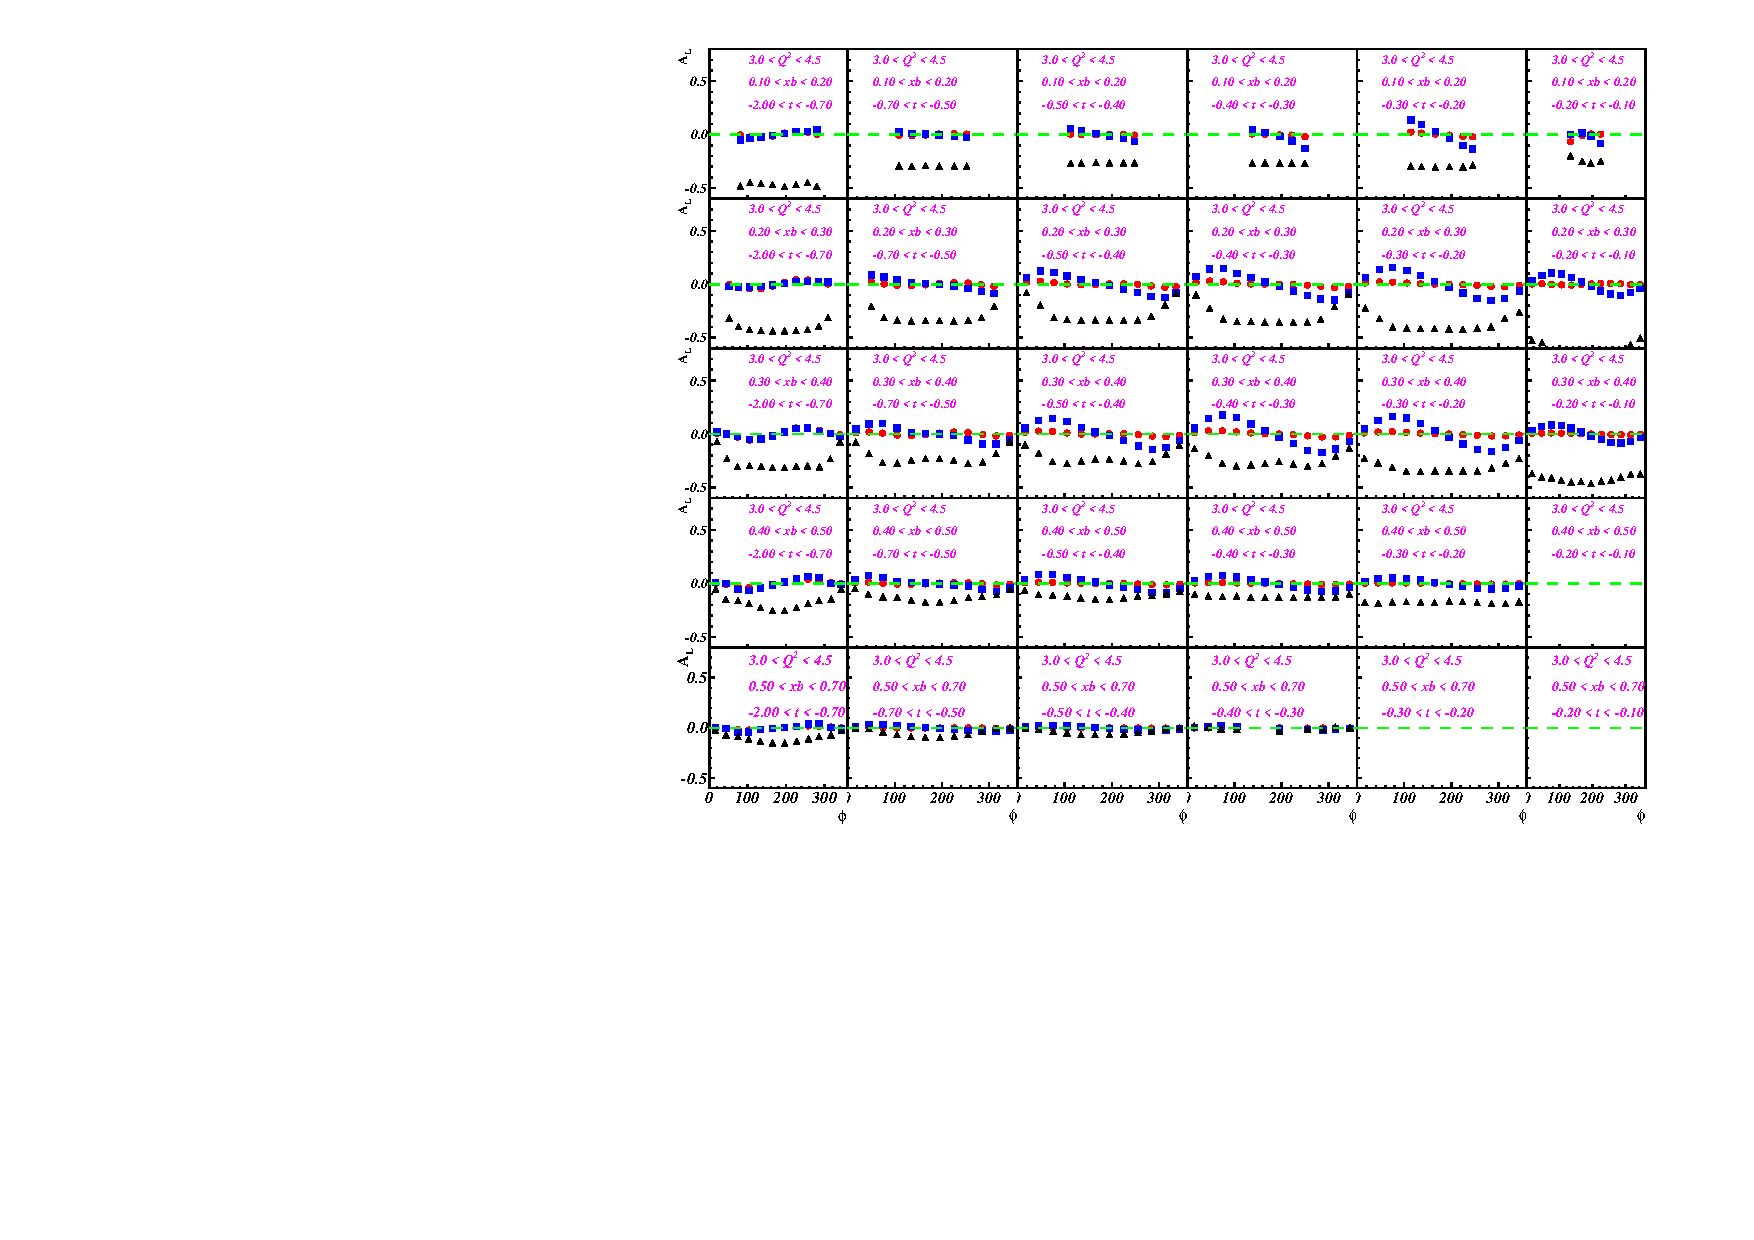
\includegraphics[width=1.\textwidth]{./figures/n_L_E11p8_Q2_3.pdf}
%   \caption[Longitudinal polarized target asymmetry distributions distribution at $E_{beam}=11~GeV$ and $Q^{2}\sim 3.5~GeV^{2}$]{\footnotesize{Longitudinal polarized target asymmetry distributions at $E_{beam}=11~GeV$ and $Q^{2}\sim 3.5~GeV^{2}$, where the red dots are $A_{LU}$, blue squares are $A_{UL}$, and black triangles are $A_{LL}$}}
%   \label{b11_Q2_3_l}
%  \end{center}
% \end{figure}
% 
%  \begin{figure}[!ht]
%  \begin{center}
%   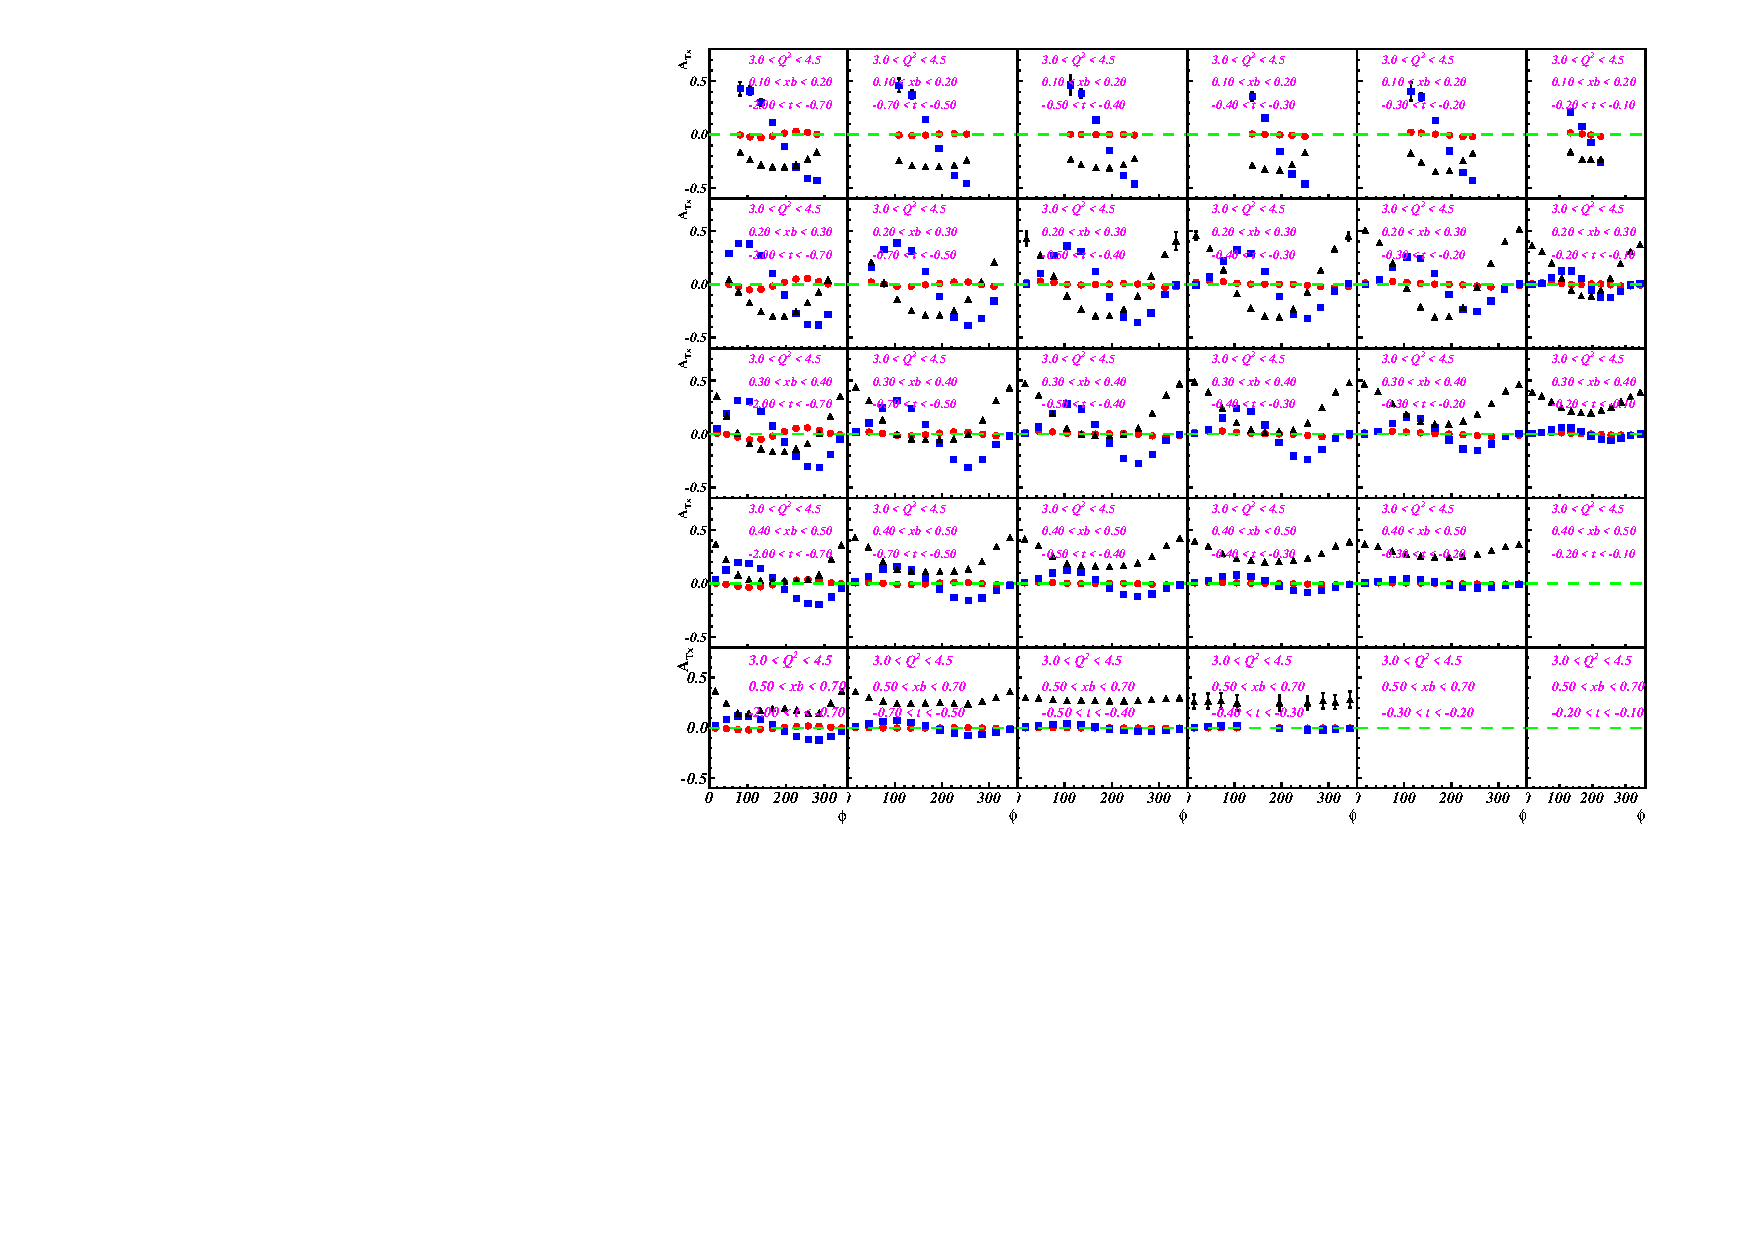
\includegraphics[width=1.\textwidth]{./figures/n_Tx_E11p8_Q2_3.pdf}
%   \caption[Transverse polarized in x target asymmetry distributions distribution at $E_{beam}=11~GeV$ and $Q^{2}\sim 3.5~GeV^{2}$]{\footnotesize{Transverse polarized in x asymmetry distributions at $E_{beam}=11~GeV$ and $Q^{2}\sim 3.5~GeV^{2}$, where the red dots are $A_{LU}$, blue squares are $A_{UTx}$, and black triangles are $A_{LTx}$}}
%   \label{b11_Q2_3_tx}
%  \end{center}
% \end{figure}
% 
%  \begin{figure}[!ht]
%  \begin{center}
%   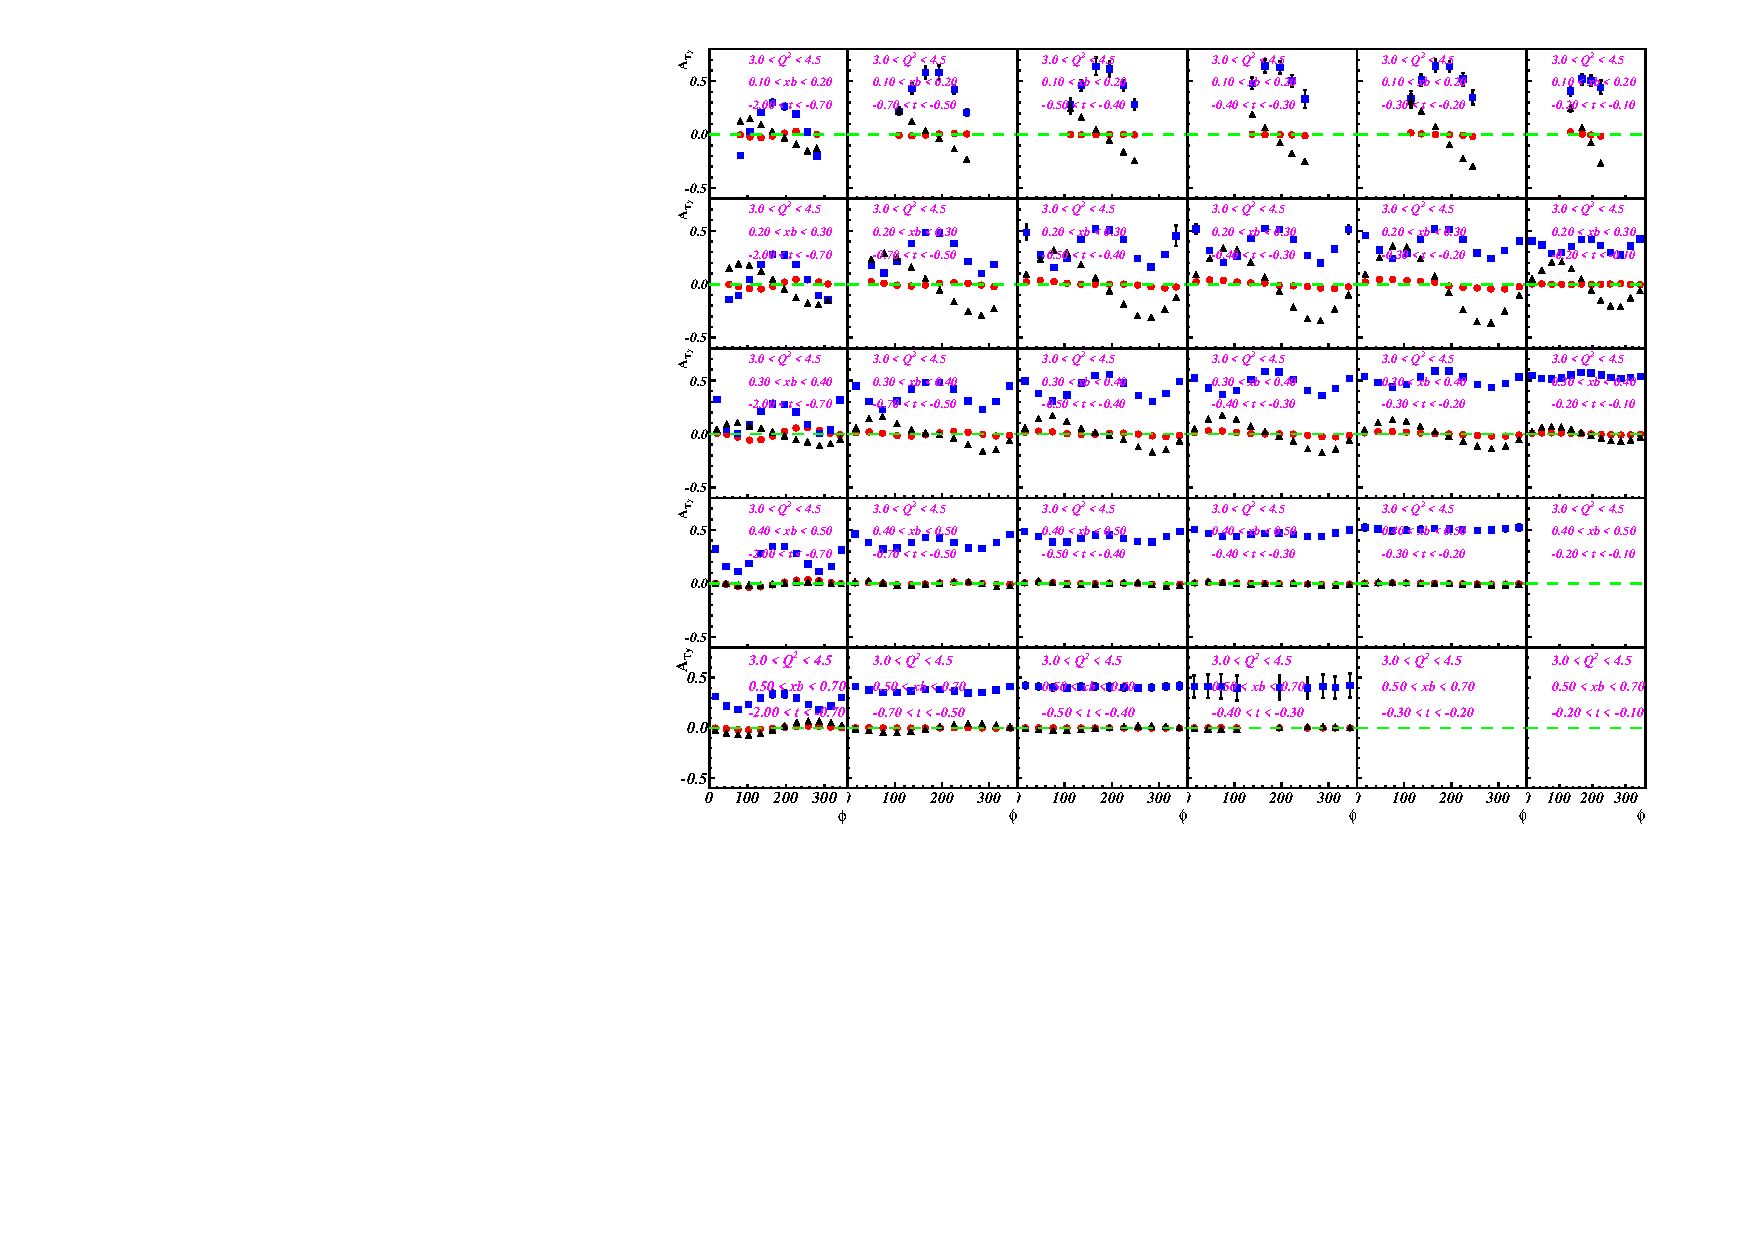
\includegraphics[width=1.\textwidth]{./figures/n_Ty_E11p8_Q2_3.pdf}
%   \caption[Transverse polarized in y target asymmetry distributions distribution at $E_{beam}=11~GeV$ and $Q^{2}\sim 3.5~GeV^{2}$]{\footnotesize{Transverse polarized in y asymmetry distributions at $E_{beam}=11~GeV$ and $Q^{2}\sim 3.5~GeV^{2}$, where the red dots are $A_{LU}$, blue squares are $A_{UTy}$, and black triangles are $A_{LTy}$}}
%   \label{b11_Q2_3_ty}
%  \end{center}
% \end{figure}
% 
% As examples, Fig.~\ref{b11_Q2_3_l}, Fig.~\ref{b11_Q2_3_tx}, and Fig.~\ref{b11_Q2_3_ty} give the distributions of $A_{BS}$, $A_{TS}$ and $A_{DS}$ as functions of $\phi$ in different $(x,t)$ combinations at $E_{beam}=11~GeV$ and $Q^{2}\sim 3.5~GeV^{2}$. The binning results results for the entire coverage can be found at: www.jlab.org\/\~yez\/Work\/DVCS\/projection.

\section{Compton Form Factor Projections}
 I am still looking for a script to fit the Compton form factors (CFF) from the asymmetry distributions as a function of $\phi$ in each ($Q^{2}, x, t$) combination. I will update the CFF projections later. 

\section{Missing Mass and Background}
 
 In the current study, we assume that we will only detect scattered electrons and real photons from the DVCS reaction, and reconstruct the neutron missing mass to select the real events. The resolutions of measuring the momentum ( or energy) and angles for electrons are determined by the GEM tracking reconstruction which is designed to achieve the following resolutions:
 \begin{equation*}
    \delta P_{e}/P_{e} \sim 2\%, \delta \theta_{e} \sim 0.6~mrad, \delta\phi_{e} \sim 5~mrad,
 \end{equation*}
and the resolutions for photons are determined by the cluster reconstruction of ECs (FAEC and LAEC). The angular resolutions are determined by the EC position resolutions and the target vertex position ($\delta z_{vertex}$) given by the electron tracking reconstruction. The current design can reach the accuracy as:
\begin{equation*}
  \delta x_{EC} = 1~cm, \delta y_{EC} = 1~cm, \delta z_{vertex} = 0.5cm.
\end{equation*}
The energy resolution of ECs is designed to be $\sim 5\%$.

The neutron missing mass spectra at the 8.8~GeV and 11~GeV setting are given in Fig.~\ref{mm_8} and Fig~\ref{mm_11}, after implemented the detector resolutions. In the same figures, the $\pi^{0}$ background was also included. However, the $\pi^{0}$ events were not weighted by their cross sections due to the lack of a working cross section model. This part is needed to be updated.

 \begin{figure}[!ht]
 \begin{center}
  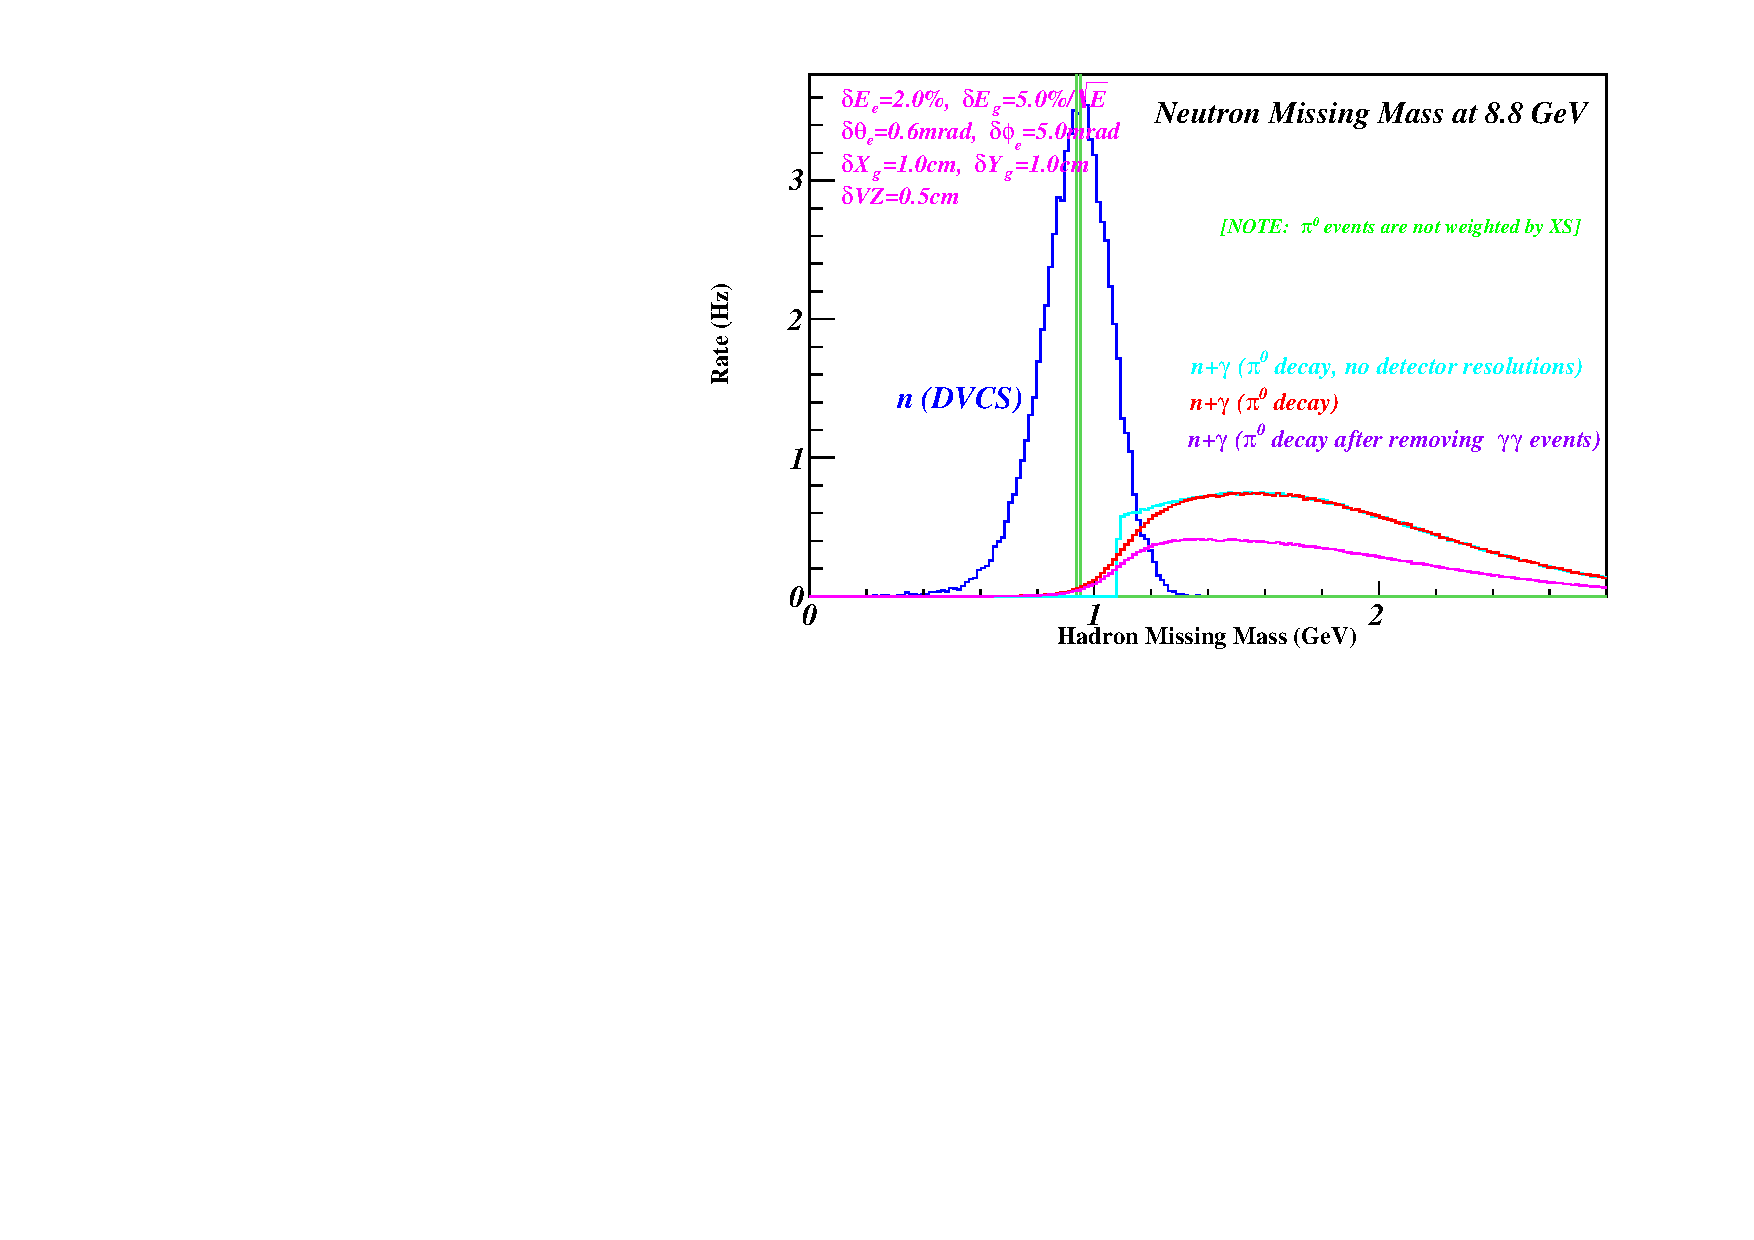
\includegraphics[width=0.6\textwidth]{./figures/neutron_DVCS_pi0_MM_8.pdf}
  \caption[The neutron missing mass at $E_{beam}=8.8~GeV$]{\footnotesize{he neutron missing mass at $E_{beam}=11~GeV$ (blue line). The detector resolutions were considered in the calculation. The $\pi^{0}$ background (red line) was normalized by comparing with the 6~GeV Hall-A DVCS results. We also evaluate the $\pi^{0}$ combination (magenta line) after removing these events which we can detect both $\pi^{0}$ decayed photons. An updated version will be available once we have the $e^{-}n\rightarrow\pi^{0}$ exclusive cross section model.}}
  \label{mm_8}
 \end{center}
\end{figure}

 \begin{figure}[!ht]
 \begin{center}
  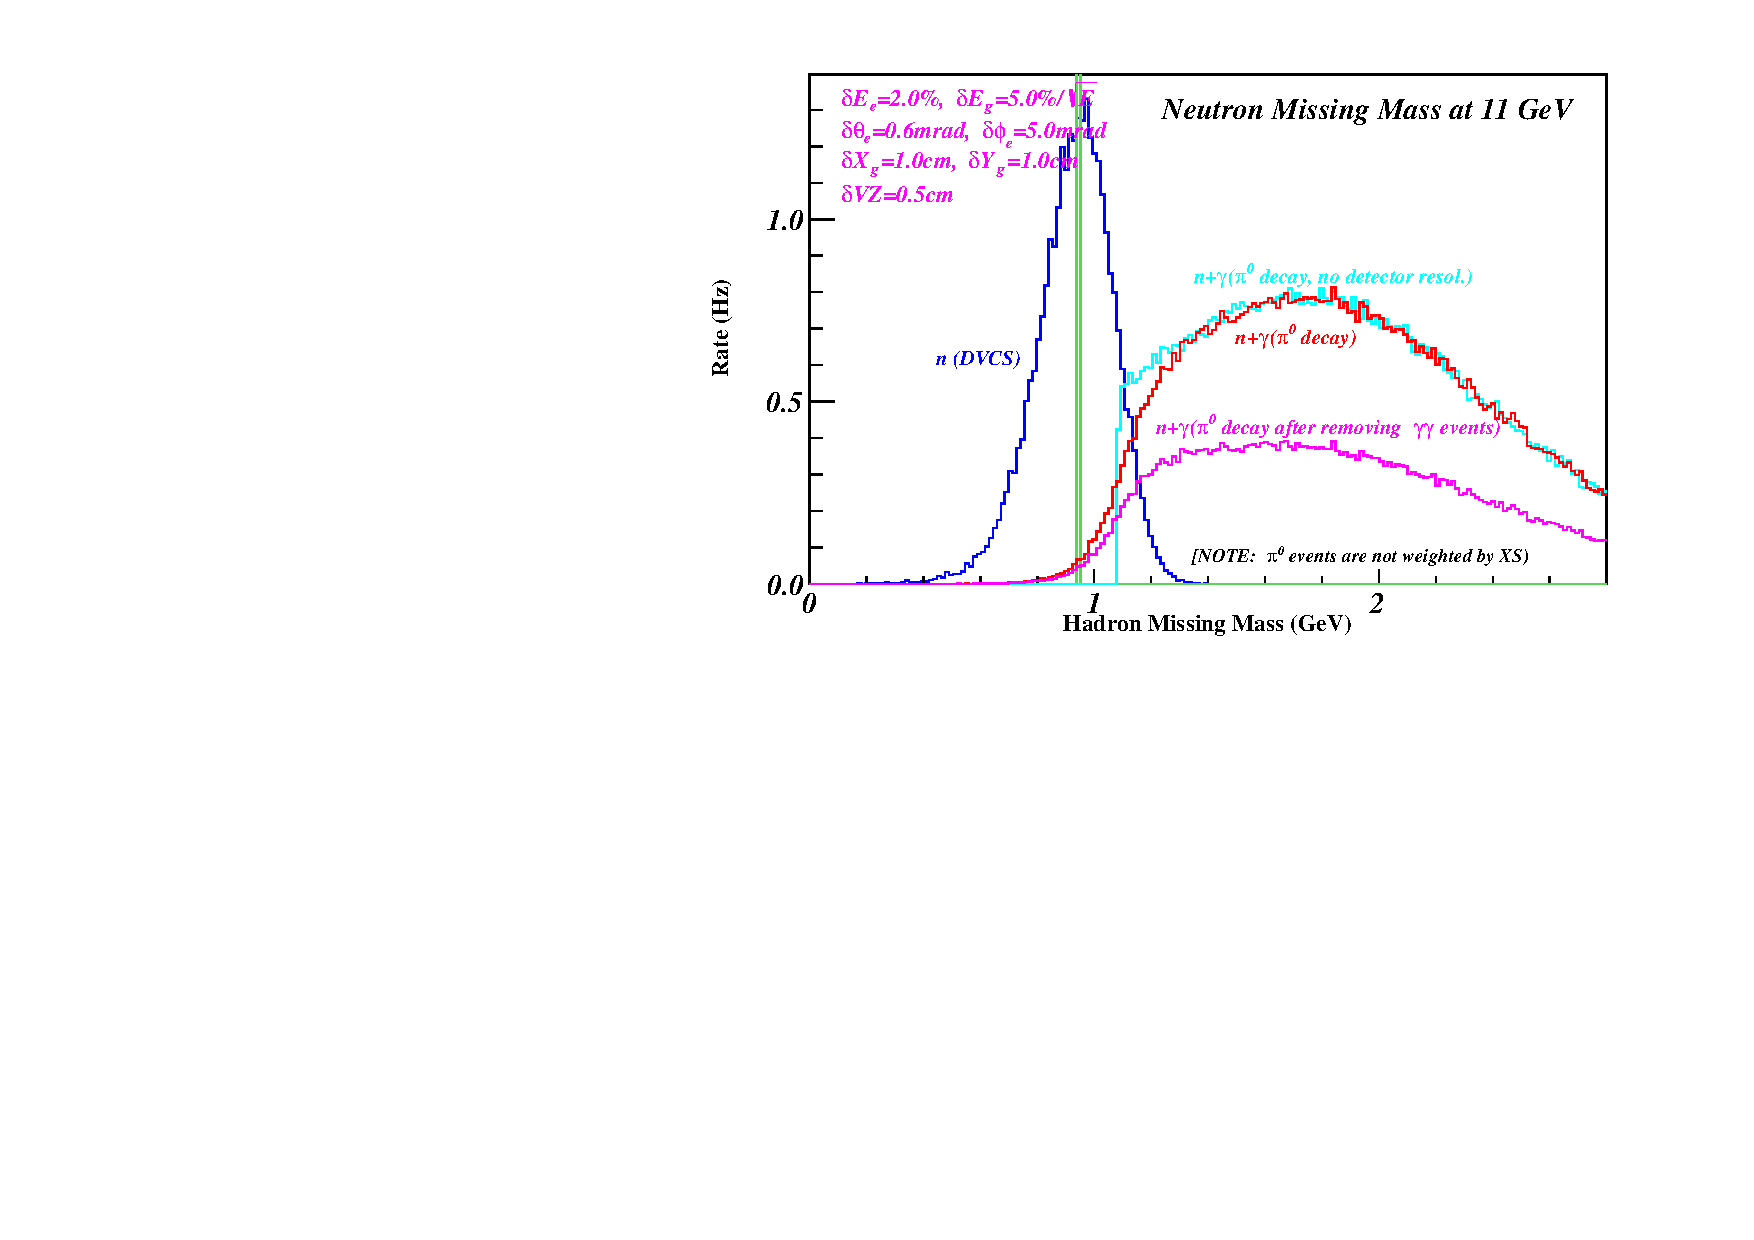
\includegraphics[width=0.6\textwidth]{./figures/neutron_DVCS_pi0_MM.pdf}
  \caption[The neutron missing mass at $E_{beam}=11~GeV$]{\footnotesize{The neutron missing mass at $E_{beam}=11~GeV$ (blue line). The detector resolutions were considered in the calculation. The $\pi^{0}$ background (red line) was normalized by comparing with the 6~GeV Hall-A DVCS results. We also evaluate the $\pi^{0}$ combination (magenta line) after removing these events which we can detect both $\pi^{0}$ decayed photons. An updated version will be available once we have the $e^{-}n\rightarrow\pi^{0}$ exclusive cross section model.}}
  \label{mm_11}
 \end{center}
\end{figure}

\end{document}          
